\subsection{Preliminaries}
\subsubsection{Volumetric Representation}
The system we present follows the familiar KinectFusion \cite{Newcombe2011} pipeline for the integration of surface information. In such a 
formulation the scene or object is represented as the zero level of a zero level set \cite{Curless1996}, where the level set is a field of distances 
to the surface and as described, the surface is given by
\begin{equation}
\begin{split}
S = \left\{\psi | \mathcal{D}(\psi) = 0\right\}
\end{split}
\end{equation}
where $S$ is the set of surface voxels, $\psi$ is a voxel in the SDF(Signed Distance Function) volume and $\mathcal{D}(.)$ is the SDF value. 
The SDF volume is truncated to yield a TSDF(Truncated Signed Distance Function) with truncation region $\mu$.

\subsubsection{Pose Estimation}
The pose estimation method used in this work is based on the ICP algorithm as used in \cite{Newcombe2011, Prisacariu2014}. The estimation of 
the camera or object 6-DoF pose is formulated as a minimisation problem of the following form
\begin{equation}
\begin{split}
E = \sum_{\omega \in \mathbf{\Omega}_{d}} \bigg( \big( \mathbf{R}\mathbf{x}_{\omega} + \mathbf{t} - \mathcal{V}(\bar{\omega}) \big)\mathcal{N}(\bar{\omega}) \bigg)^{2}
\end{split}
\end{equation}
where $\mathbf{\Omega}_{d}$ is a depth image, $\omega$ is a 3D point extracted form the depth image, $\mathbf{R}$ is an  $\mathbbm{SO}(3)$ 
rotation matrix, $\mathbf{t}$ is a translation vector, $\mathcal{V}$ is a rendered depth map from the SDF model, $\mathcal{N}$ is a rendered 
normal map from the SDF model and $\bar{\omega}$ is the point $\omega$ projected into the coordinate frame of $\mathcal{V}$ and 
$\mathcal{N}$.

\subsection{Surface Integration}
As in previous works \cite{Newcombe2011,Prisacariu2014} we utilise a weighted mean to fuse new depth measurements in to the TSDF model. As such, 
for a new depth measurement $\eta$ projected to by voxel $\psi$, the following update to the TSDF volume $\mathcal{D}$ is made
\begin{equation}
\begin{split}
\mathcal{D}'(\psi) \leftarrow \frac{w(\psi)\mathcal{D}(\psi) + \min(1, \eta/\mu)}{w(\psi) + 1}
\end{split}
\end{equation}
where $w(.)$ is a weighting function and $\mu$ is the aforementioned TSDF truncation region.

\subsection{Representation and Fusion Procedure}
The representation of the object to be reconstructed makes use of multiple `subvolumes' each pertaining to some patch on the object surface. 
New subvolumes are started when a sufficient amount of new voxels have been allocated and have had data integrated. By ensuring overlap 
between the subvolumes, transformations between them can be found. Using the multiple volume approach allows for pose estimation in each 
volume such that pose estimation discrepancies between subvolumes can be detected and are indicative of pose estimation drift.

The proposed system is inspired by\cite{Kolev2006} in that the representation used for the shape of the object to be modelled is a set of volumes 
of probabilities and surface information. The probabilities are posteriors over a per voxel assignment to either the object voxel set or to the non 
object voxel set. In the proposed system this volume of posterior probabilities is built into with each frame, parallel to the fusion process in systems 
such as KinectFusion\cite{Newcombe2011} and InfiniTAM\cite{Prisacariu2014}.

At each frame a probability map is constructed based on the predictions of the model given the current frame. During the fusion process, this 
smaller volume is mapped in to as a source of voxel wise appearance probability information. The overall appearance based posterior for a given voxel 
$\psi \in \mathbf{\Psi}$ takes the following form:
\begin{equation}
\begin{split}
P(\psi \in \mathbf{\Phi} | \mathbf{\Omega}, \mathbf{p}) = \prod_{t=0}^{\infty} P(\psi_{t} \in \mathbf{\Phi}_{t} | \mathbf{\Omega}_{t}, \mathbf{p}_{t})
\end{split}
\end{equation}
where $\mathbf{\Psi}$ is the volume of voxels for which measurements are accumulated, $\mathbf{\Phi}$ 
is the volume of voxels pertaining to the object, $\mathbf{\Omega}_{t}$ is the current image observation at time $t$ and $\mathbf{p}_{t}$ is the 
currently tracked pose at time $t$.
The above encodes the probability of a voxel belonging to an object as the product of the instantaneous conditionals for observations at each time step. 
Note that in general $\mathbf{\Phi} \subset \mathbf{\Psi}$, and the use of $\mathbf{\Phi}$ in the above equation is an abuse of notation as in the above 
$\mathbf{\Phi}$ is a discretisation of the continuous $\mathbf{\Phi}$ in the probabilistic formulation that follows. Finally, note that a conditional 
independence assumption is made to aid computational tractability in the model.

\subsection{Probabilistic Formulation of Object Reconstruction}
As previously highlighted, central to the proposed system is a volume of posterior probabilities pertaining to a voxel wise membership of either the 
object set or the non object set. This allows one to formulate the full joint distribution over the object as the Probabilistic 
Graphical Model of Figure \ref{pgm1}.
\begin{figure}[h]
	\centering
	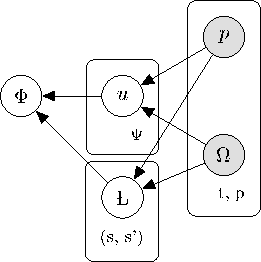
\includegraphics{graphical_models/pgm1.pdf}
	\caption{Probabilistic formulation of the object reconstruction pipeline.}
	\label{pgm1}
\end{figure}

Where $\mathbf{\Phi}$ is the shape to be reconstructed, $\mathbf{u}$ is the appearance model volume, $\mathbf{L}$ is the 
set of consistency constraints for each adjacent sub volume pair in the form of rigid transformations, $\mathbf{\Omega}$ is the set of 
RGBD image pixels and $\mathbf{p}$ the set of poses over time.

This gives rise to the following analytical formulation of the above distribution:

\begin{equation}
\begin{split}
P(\mathbf{\Phi}, \mathbf{\Omega}, \mathbf{p}, \mathbf{u}, \mathbf{L}) = 
\prod_{\psi \in \mathbf{\Psi}}\prod_{(s, s') \in \mathcal{S}}P(\mathbf{\Phi}|\mathbf{u}_{v}, \mathbf{L}_{(s, s')}) 
\prod_{t=0}^{\infty}\prod_{p \in \mathcal{P}}\\
P(\mathbf{u_{v}}|\mathbf{\Omega}_{p, t}, \mathbf{p}_{t})
P(\mathbf{L}_{(s, s')}|\mathbf{\Omega}_{p, t}, \mathbf{p}_{t})
P(\mathbf{L}_{(s, s')})P(\mathbf{p}_{t})P(\mathbf{\Omega}_{p, t})
\end{split}
\end{equation}
where $\mathcal{V}$ is the set of voxels across all sub volumes, $\mathcal{P}$ is the set of RGBD pixels for a given 
frame and $\mathcal{S}$ is the set of sub volumes.

However, if one were to assume temporal and pixel wise independence in the RGBD observations and temporal independence in 
the poses, the plate containing $\mathbf{\Omega}$ and $\mathbf{p}$ can be removed:
\begin{equation}
\begin{split}
P(\mathbf{\Phi}, \mathbf{\Omega}, \mathbf{p}, \mathbf{u}, \mathbf{L}) = 
\prod_{v \in \mathcal{V}}P(\mathbf{\Phi}|\mathbf{u}_{v})
\prod_{(s, s') \in \mathcal{S}}P(\mathbf{u_{v}}|\mathbf{\Omega}, \mathbf{p}, \mathbf{L}_{(s, s')})\\
P(\mathbf{L}_{(s, s')}|\mathbf{\Omega}, \mathbf{p}) P(\mathbf{L}_{(s, s')})P(\mathbf{p})P(\mathbf{\Omega})
\end{split}
\end{equation}
In practice this temporal independence assumption causes no issues.

Furthermore, if one assumes voxel wise independence, the plate over voxels can be removed. Finally, assuming $P(\mathbf{p})$ and 
$P(\mathbf{\Omega})$ are uniform distributions, then we have the simpler distribution given by Figure \ref{pgm2}.
\begin{figure}[h]
	\centering
	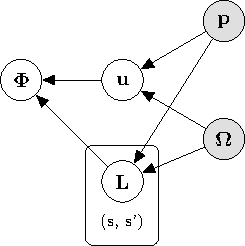
\includegraphics{graphical_models/pgm2.pdf}
	\caption{Simplified probabilistic formulation of the object reconstruction pipeline.}
	\label{pgm2}
\end{figure}

Where the simpler distribution takes the following analytical form:
\begin{equation}
\begin{split}
P(\mathbf{\Phi}, \mathbf{\Omega}, \mathbf{p}, \mathbf{u}, \mathbf{L}) = 
\prod_{(s, s') \in \mathcal{S}} P(\mathbf{\Phi}|\mathbf{u}, \mathbf{L}_{(s, s')})
P(\mathbf{u}|\mathbf{\Omega}, \mathbf{p})\\
P(\mathbf{L}_{(s, s')}|\mathbf{\Omega}, \mathbf{p})
P(\mathbf{L}_{(s, s')})
\end{split}
\end{equation}

The above formalisms describe a probabilistic framework in which online corrections can be made to the reconstructed model to counteract 
errors incurred by pose tracking inconsistencies. As with previous dense SLAM systems \cite{Newcombe2011, Prisacariu2014, Niessner2013}, 
our system follows a pipeline that consists of a tracking stage and an integration stage. However, our formulation of this pipeline 
consists of an additional estimation module that relies on the use of a subvolume representation to correct tracking errors by applying 
transformations to the subsegments to align them when there are intra subsegment tracking inconsistencies. 
As previously described, during reconstruction the object is split in to subsegments, also referred to as subvolumes, 
with the pose estimation performed in each of the active, visible subsegments. The pose estimation stage for each of these subsegments follows 
the standard ICP(Iterated Closest Point) approach.
As inference on the joint distribution of our model is intractable, conditional independence assumptions are made that do not appear 
to cause any functional issues. The estimation phase of the pipeline is described in the following section.

\subsection{Estimating Deformations}
The tracking consistency constraint denoted by the variable $\mathbf{L}$ in the graphical model given by Figure \ref{pgm1} and Figure \ref{pgm2} can 
be enforced in terms of minimising the transformations between adjacent submaps, such that the camera poses tracked in each subvolume are consistent.  
%The approach proposed in this work differs from \cite{Kahler2016} in that the optimisation is integrated in to the probabilistic formulation previously outlined. 
Given instantaneously inferred transforms between subvolumes obtained from tracking results, 
the objective is to infer a robust, consistent deformation transformation for the subvolume pair.

As such, for each pair of visible subvolumes $(s, s')$, the following posterior must be maximised:
\begin{equation}
\begin{split}
%Bayes rule + chain rule for P(omega, p)
P(\mathbf{\Omega}, \mathbf{p} | \mathbf{L}_{(s, s')}) = \frac{P(\mathbf{L}_{(s, s')} | \mathbf{\Omega}, \mathbf{p}) P(\mathbf{\Omega} | \mathbf{p})P(\mathbf{p})}
{P(\mathbf{L}_{(s, s')})}
\end{split}
\end{equation}
The intuition behind the above equation is that the deformation $\mathbf{L}_{(s, s')}$ applied to the probability field $\mathbf{u}$ should 
increase the probability of observing the current pose $\mathbf{p}$ given the current RGBD frame $\mathbf{\Omega}$ by reducing the 
variance of the camera tracking result. As such, global tracking variance is reduced by enforcing local consistency, improving the quality 
of the reconstruction.

A gradient based maximisation of the above posterior to yield an optimal deformation is a highly nonlinear optimisation problem. As such, it is suited 
to second order gradient based optimisation routines such as Gauss-Newton or Levenberg-Marquardt.
It should be noted that in our implementation the $P(\mathbf{\Omega} | \mathbf{p})$ term is assumed to be uniform in the case of an 
RGBD sensor being used, however for applications such as monocular SLAM this term may be replaced with a noise model when there is 
significant uncertainty about the given depth map at each frame.

The following proportionality to the distribution over deformations is made:
\begin{equation}
\begin{split}
P(\mathbf{L}_{(s, s')} | \mathbf{\Omega}, \mathbf{p}) \propto P(\mathbf{\Psi}_{s}(\mathbf{x}) | \mathbf{\Psi}_{s'}(\Lambda(\mathbf{x})))
\end{split}
\end{equation}
With the likelihood function taking the following form:
\begin{equation}
\begin{split}
P(\mathbf{\Psi}_{s'}(\Lambda(\mathbf{x}))) = \prod_{(s, s') \in \mathcal{S}} \frac{1}{\sqrt{2 \pi \sigma}} \exp{\frac{-(\mathbf{\Psi}_{s}(\mathbf{x}) - \mathbf{\Psi}_{s'}(\Lambda(\mathbf{x})))^2}{2\sigma^2}}
\end{split}
\end{equation}
Or alternatively:-
\begin{equation}
\begin{split}
\ln P(\mathbf{\Psi}_{s'}(\Lambda(\mathbf{x}))) = m\ln\frac{1}{\sqrt{2\pi}\sigma}\\
-\frac{1}{2\sigma^2} \sum_{(s, s') \in \mathcal{S}} \bigg( \mathbf{\Psi}_{s}(\mathbf{x}) - \mathbf{\Psi}_{s'}(G(\mathbf{x})) \bigg)^2
\end{split}
\end{equation}
Where $\mathbf{\Psi}(.)$ is a scalar valued SDF(Signed Distance Function), a dicretised field of $\mathbf{\Phi}$, as previously described. $\mathbf{x}$ is a point represented by a 3-vector and $\Lambda(.)$ is a transformation function taking the following form:
\begin{equation}
\begin{split}
\Lambda(\mathbf{x}) = \mathbf{R}(r_{1}, r_{2}, r_{3})\mathbf{x} + \mathbf{t}
\end{split}
\end{equation}
Where $\mathbf{R}(.)$ is a rotation matrix from the Special Orthogonal group $\mathbbm{SO}(3)$ paramaterised by the three 
Rodrigues Parameters\cite{Shuster1993} $r_{1}$, $r_{2}$ and $r_{3}$.

Note that the logarithmic form of the above likelihood is suitable to Nonlinear Least Squares optimisation, allowing the posterior of equation 4 
to be maximised in terms of the likelihood term of equation 4. To perform MLE(Maximum Likelihood Estimation) over this likelihood using 
an optimisation routine such as Levenberg Marquardt, the following gradients must be computed for the rotational component of the 
deformation:-
\begin{equation}
\begin{split}
\frac{\partial E}{\partial r_{n}} = \frac{\partial E}{\partial \mathbf{\Psi}} \frac{\partial \mathbf{\Psi}}{\partial \Lambda} \frac{\partial \Lambda}{\partial r_{n}} \text{for } n \in \{1,2,3\}
\end{split}
\end{equation}
Similarly for the translational component:-
\begin{equation}
\begin{split}
\frac{\partial E}{\partial \mathbf{t}_{d}} = \frac{\partial E}{\partial \mathbf{\Psi}} \frac{\partial \mathbf{\Psi}}{\partial \Lambda} \frac{\partial \Lambda}{\partial \mathbf{t}_{d}} \text{for } d \in  \{x,y,z\}
\end{split}
\end{equation}
where the gradient $\frac{\partial \mathbf{\Psi}}{\partial \Lambda}$ is found via finite differencing.

\section{Implicit Surface Deformations}
In the previous section, a model and estimation procedure was presented to find optimal transformations between the aforementioned subvolumes.
The overall object surface $\mathbf{\Phi}$ is implicitly deformed by a combining function $\mathbf{\zeta}(\mathbf{\Phi})$ over each of the subvolumes to which transformations have been applied.
As such the surface $\mathbf{\Phi}$ is given by the following:
\begin{equation}
\begin{split}
\mathbf{\Phi} = \int_{\chi \in X} \mathbf{\zeta}(\mathbf{\Phi}_{\chi}) d \mathbf{\Phi}_{\chi}
\end{split}
\end{equation}
where $X$ is the set of subvolumes contributing to the surface $\mathbf{\Phi}$.

As such, the previously described transformation estimation process that deforms each of the subscenes implicitly to optimise jointly for the true 
surface as depicted in Figure.
\begin{figure*}[!t]
	\centering
	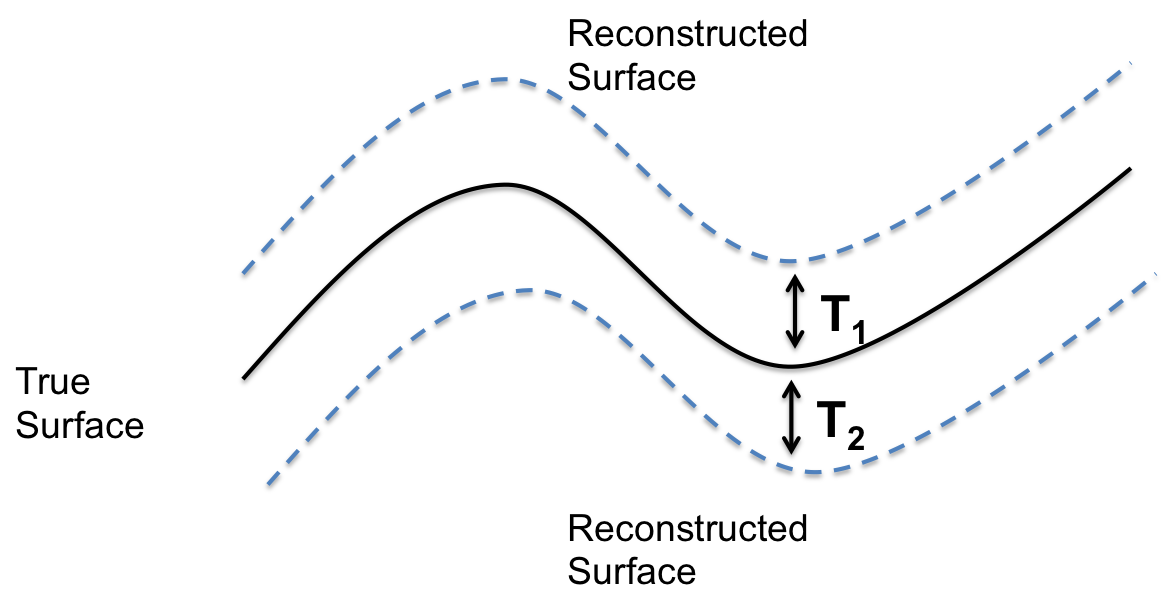
\includegraphics[scale=0.25]{deformation.png}
	\caption{Measured surfaces being deformed to the true surface.}
	\label{deformationDiagram}
\end{figure*}


\section{Volumetric Object Segmentation}
The final stage in the proposed object reconstruction pipeline is the segmentation of the object voxels from those that have had measurements fused 
from the background. This segmentation is formulated within a CRF framework, where each node in the CRF represents a set of neighbouring voxels in space, 
with connections being made between adjacent neighbourhoods. The process of segmentation can be posed as an energy minimisation problem over a cut in voxel space, 
such that a segmentation in 3D is obtained. The following energy function consists of the unary posterior probabilities over appearance accumulated during the fusion 
process for a region in space and an additional pairwise smoothing term representing the physical appearance similarity of the object region represented by the voxel 
neighbourhoods $\gamma$ and $\gamma^{'}$:
\begin{equation}
\begin{split}
E_{n} = \prod_{t=0}^{\infty} \prod_{\psi \in \mathbf{\Phi}_{n}} P(\psi \in \mathbf{\Psi} | \mathbf{\Omega}_{t}, \mathbf{p}_{t}) + P(\mathbb{E}[\mathbf{c}]_{\gamma} | \mathbb{E}[\mathbf{c}]_{\gamma^{'}})
\end{split}
\end{equation}
where $\mathbf{c}$ represents the set of colour measurements fused in to the voxels within a given neighbourhood, for all $N$ subvolumes.

\section{Implementation Notes}
The probabilities that are accumulated into the volume are generated from a Random Forest based appearance model using patch based features encompassing 
appearance and surface information, such as depth gradients, initialised prior to reconstruction by a user interaction in the first frame. There are two 
classes in the appearance model, one for the foreground object and one for the background, with the foreground object indicated by a bounding box on the 
first RGB frame.

An overview of the processing pipeline for the proposed system is outlined in Figure \ref{pipelineDiagram}.
\begin{figure*}[!t]
	\centering
	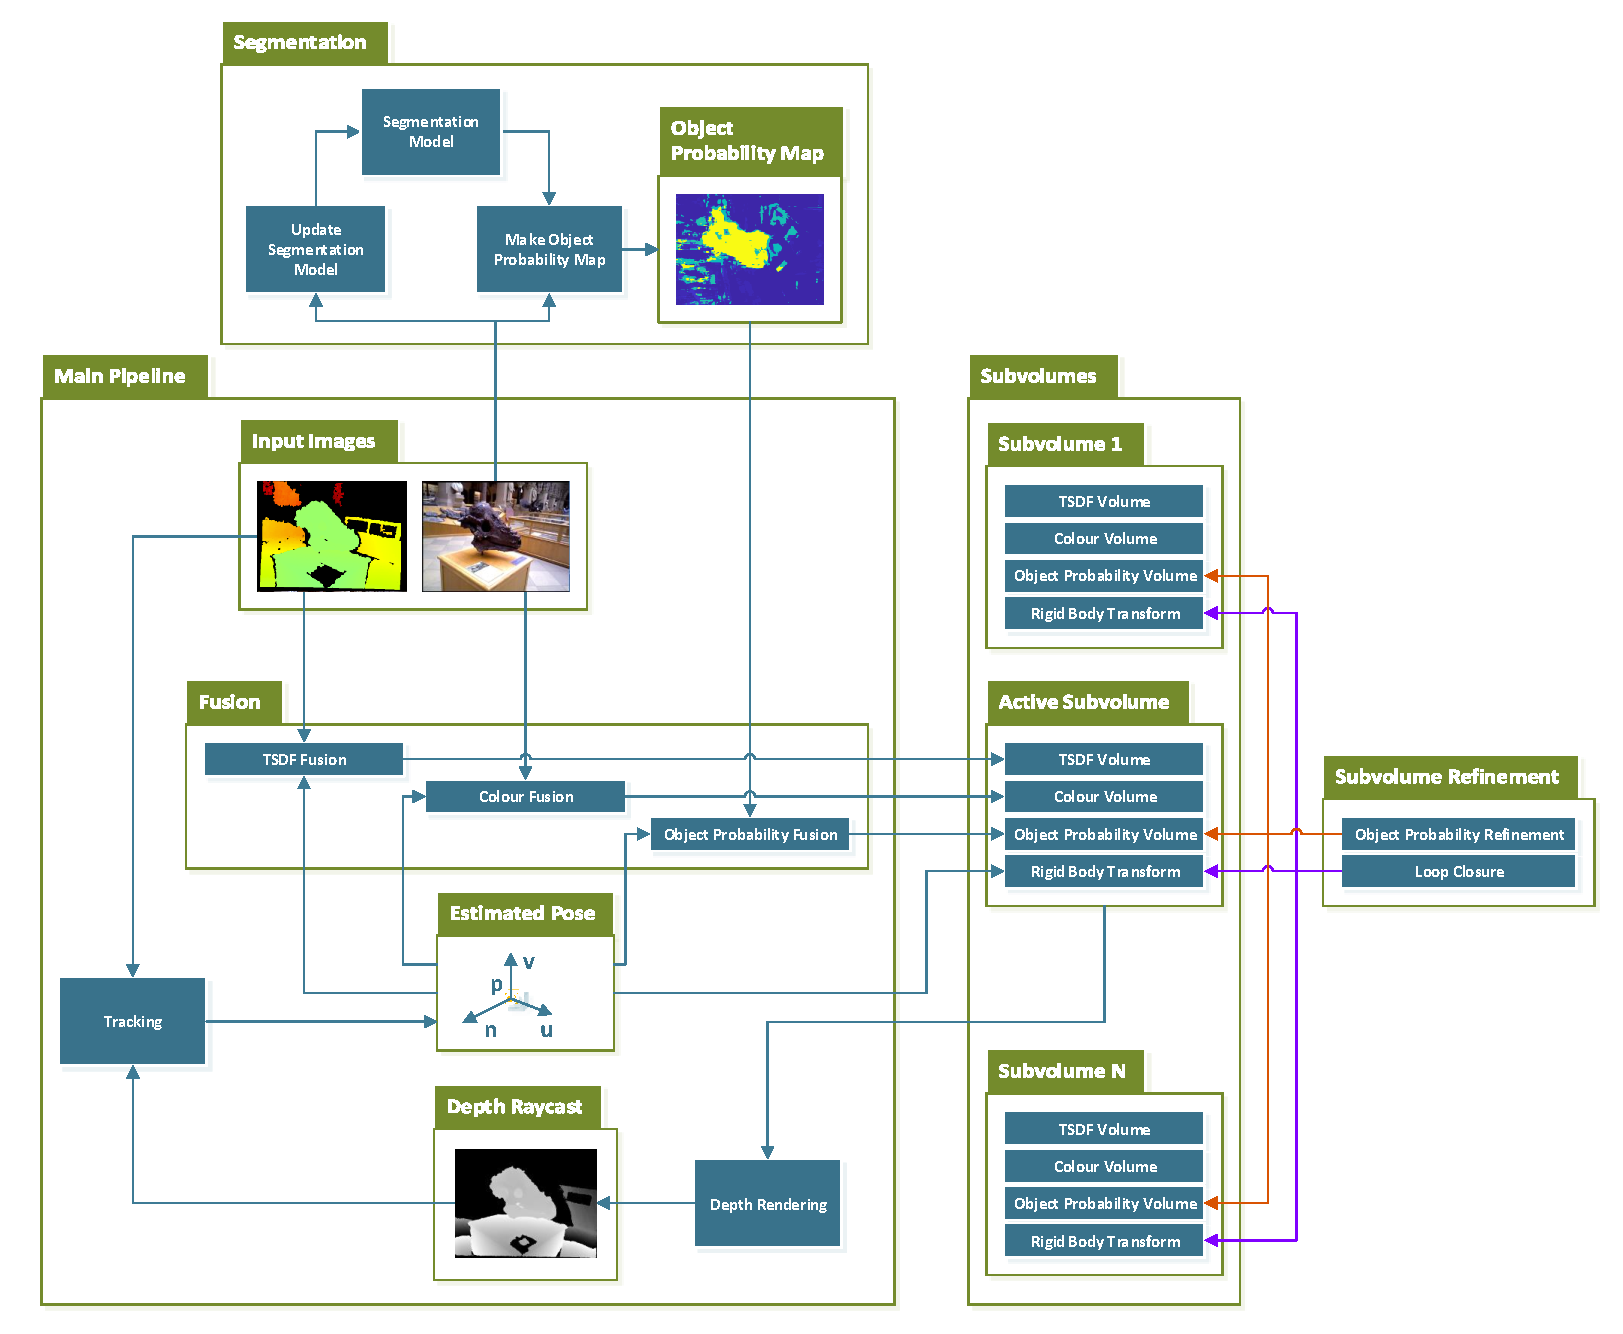
\includegraphics[scale=0.5]{pipeline.pdf}
	\caption{Object reconstruction pipeline.}
	\label{pipelineDiagram}
\end{figure*}